\documentclass{beamer}
\usepackage{lmodern}
\usepackage{siunitx}
\usepackage[version=3]{mhchem}
\graphicspath{{material/}{material/nue_H1/}{material/nue_C12/}}

\newcolumntype{C}{>{\centering\arraybackslash} m{0.1cm} }  %# New column type
\newcolumntype{V}{>{\centering\arraybackslash} m{0.45\linewidth} }

\title{Neutrino Directionality}
\subtitle{Test with KLG4}
\author[Michinari]{Michinari Sakai}
%\date

\begin{document}

\frame{\titlepage}

\begin{frame}
	\frametitle{Agreement between true/reconstructed $\nu$ angle}
	\framesubtitle{no fiducial volume cut}
	\begin{columns}[T]
		\column{0.5\textwidth}
		\ce{\nu_{e} + ^{1}H -> e^{-} + ?}
		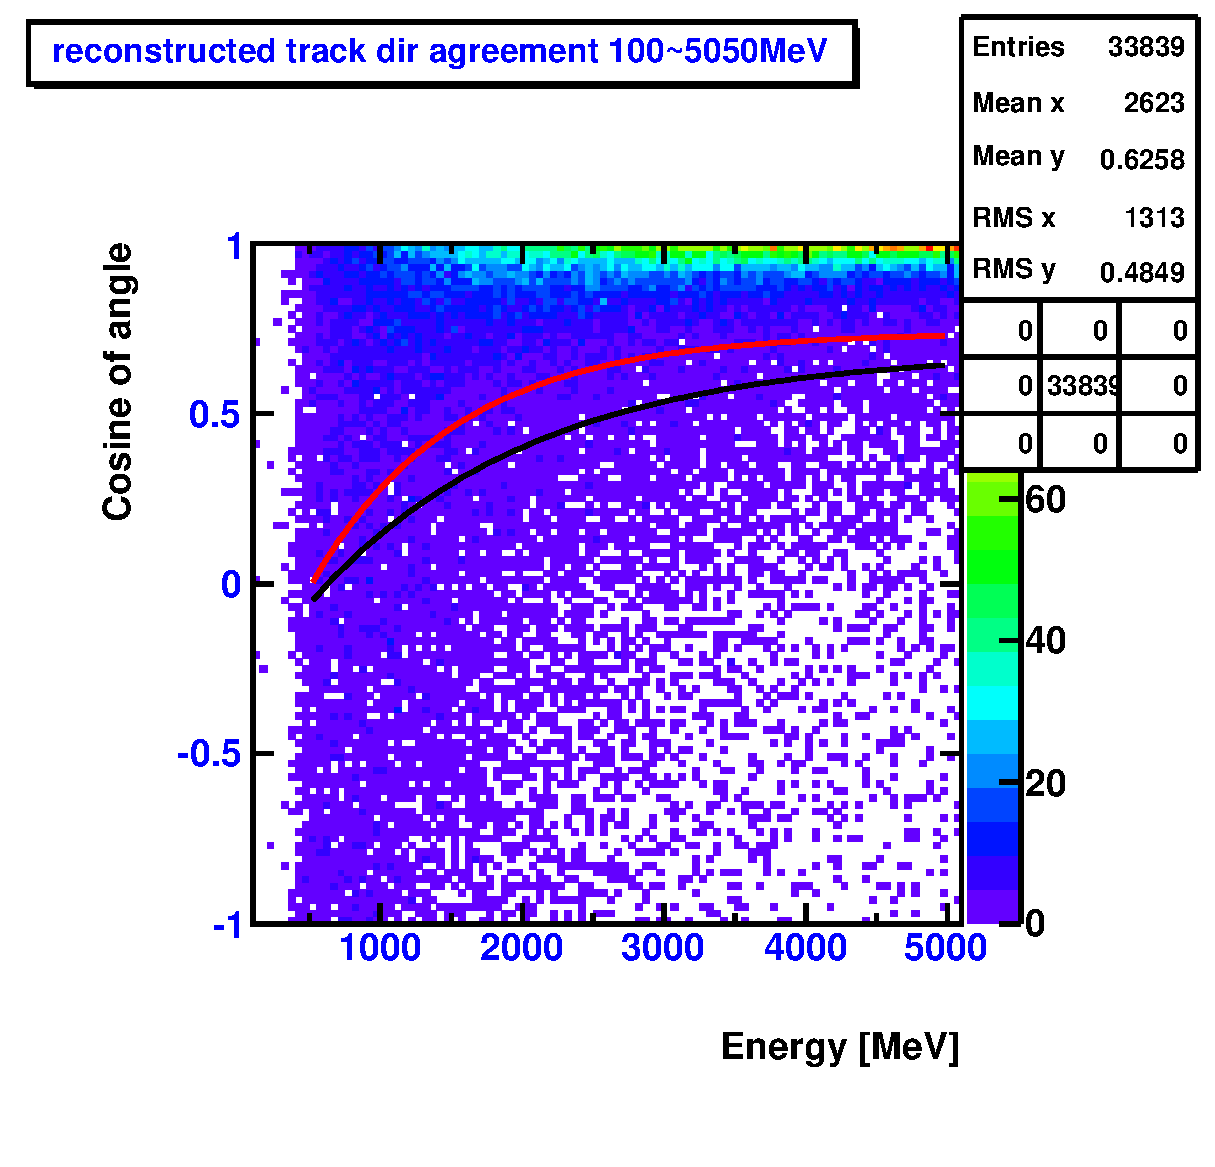
\includegraphics[width=1.0\textwidth]{analyzed_mtq_flatSpectrum_nue_H1_outerBufferFillAll_reconDirAgreementWithMtqTruthVectorVSEnergy_onlyCC.eps}
		\column{0.5\textwidth}
		\ce{\nu_{e} + ^{12}C -> e^{-} + ?}
		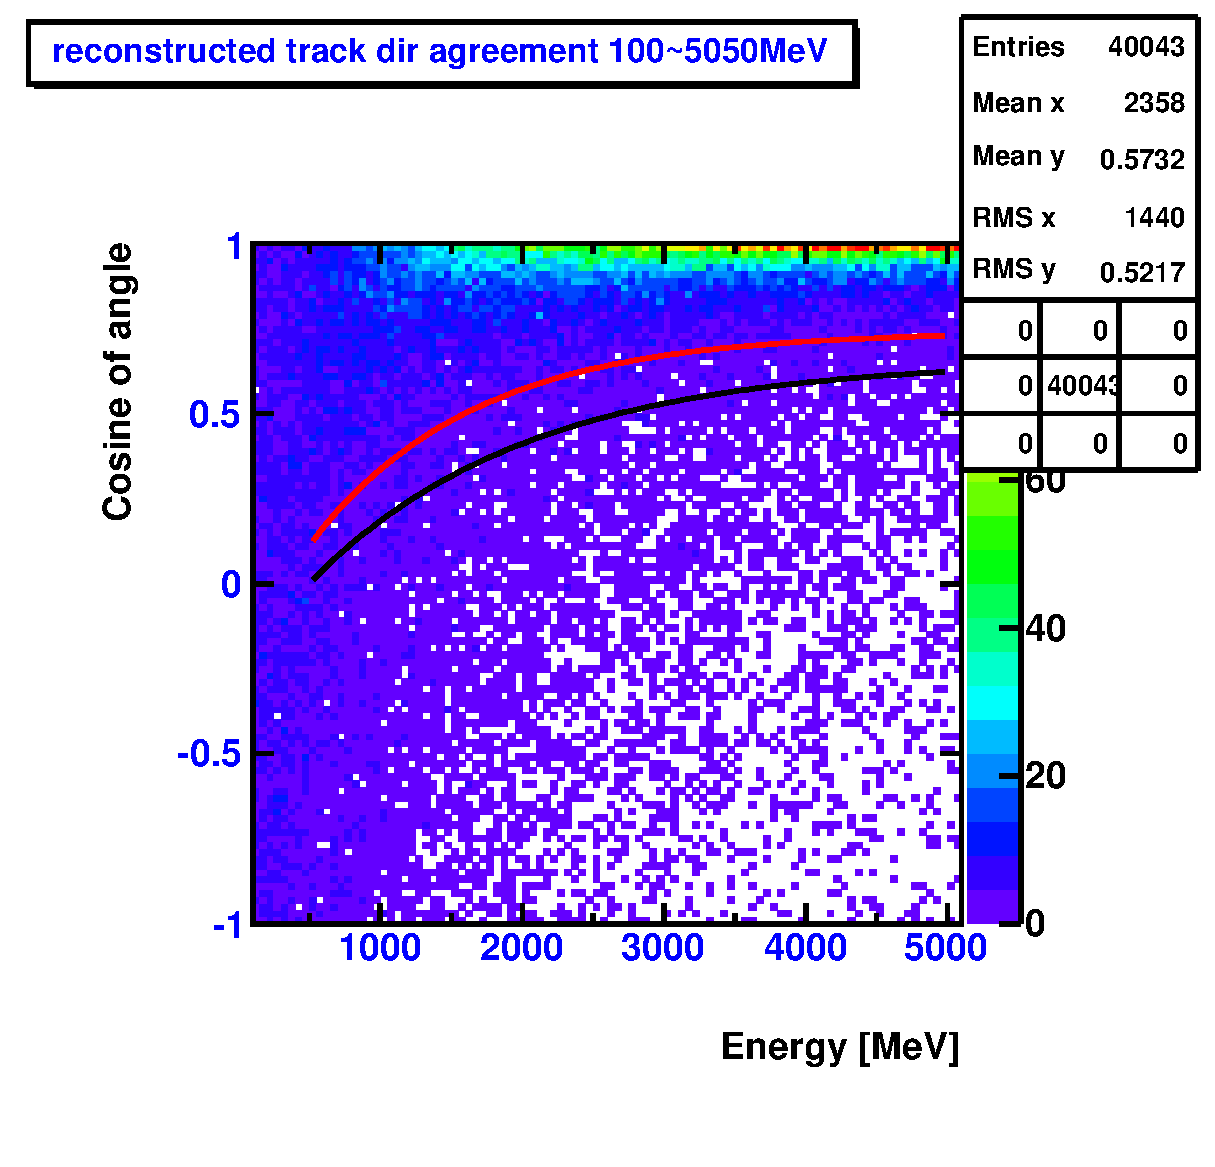
\includegraphics[width=1.0\textwidth]{analyzed_mtq_flatSpectrum_nue_C12_outerBufferFillAll_reconDirAgreementWithMtqTruthVectorVSEnergy_onlyCC.eps}
	\end{columns}
\end{frame}

\begin{frame}
	\frametitle{Agreement between true/reconstructed $\nu$ angle}
	\framesubtitle{vertex $R < \SI{600}{cm}$}
	\begin{columns}[t]
		\column{0.5\textwidth}
		\ce{\nu_{e} + ^{1}H -> e^{-} + ?}
		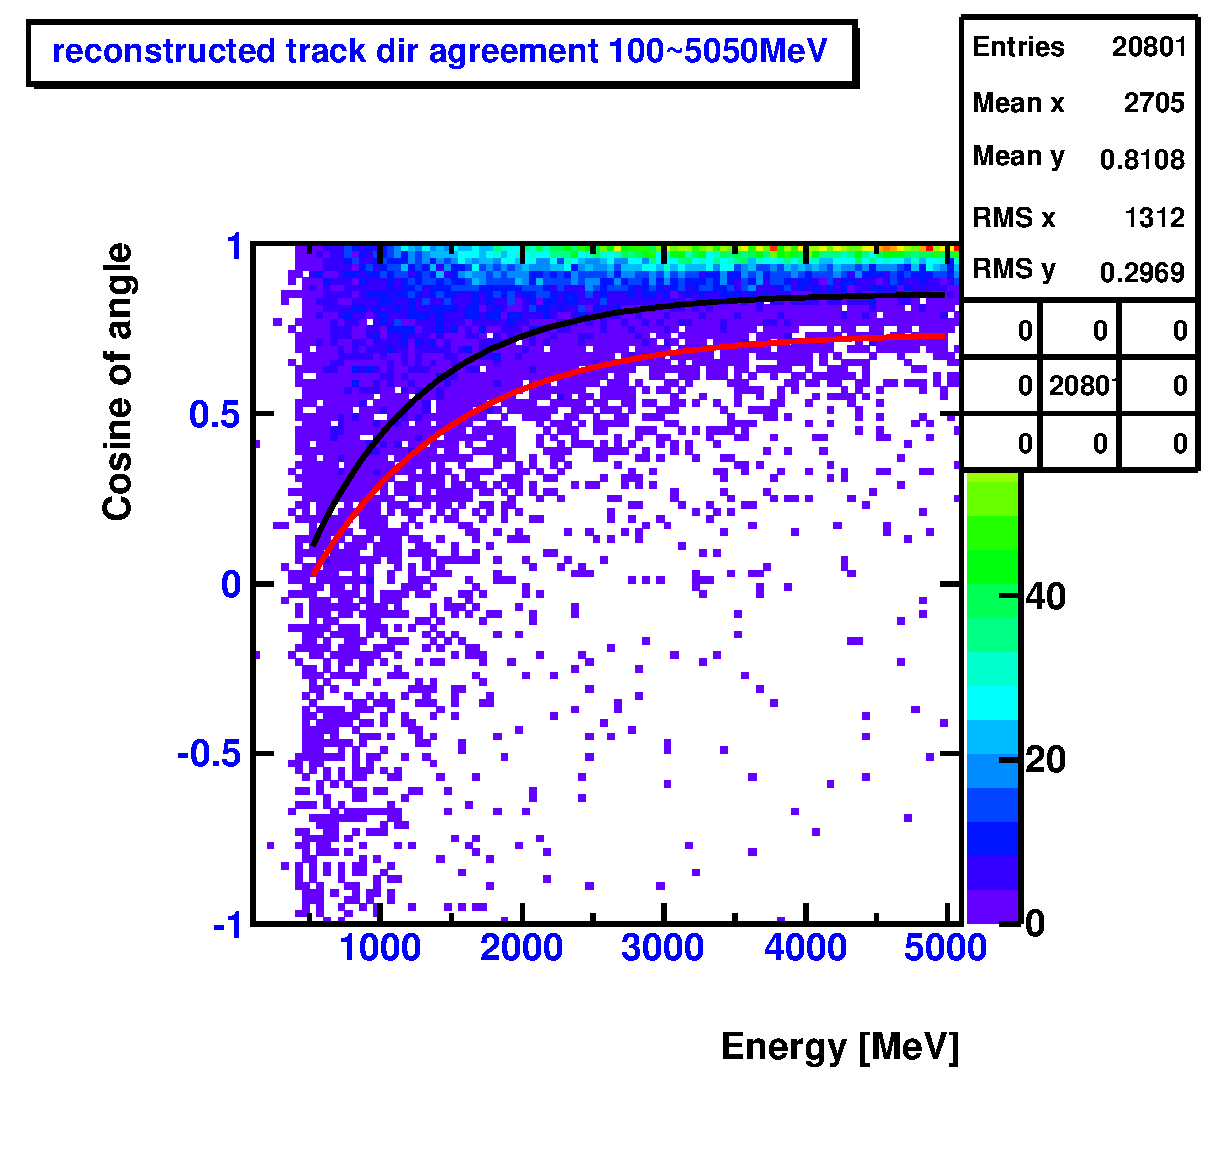
\includegraphics[width=1.0\textwidth]{material/nue_H1/analyzed_mtq_flatSpectrum_nue_H1_outerBufferFillAll_reconDirAgreementWithMtqTruthVectorVSEnergy_onlyCC_maxR600cm.eps}
		\column{0.5\textwidth}
		\ce{\nu_{e} + ^{12}C -> e^{-} + ?}
		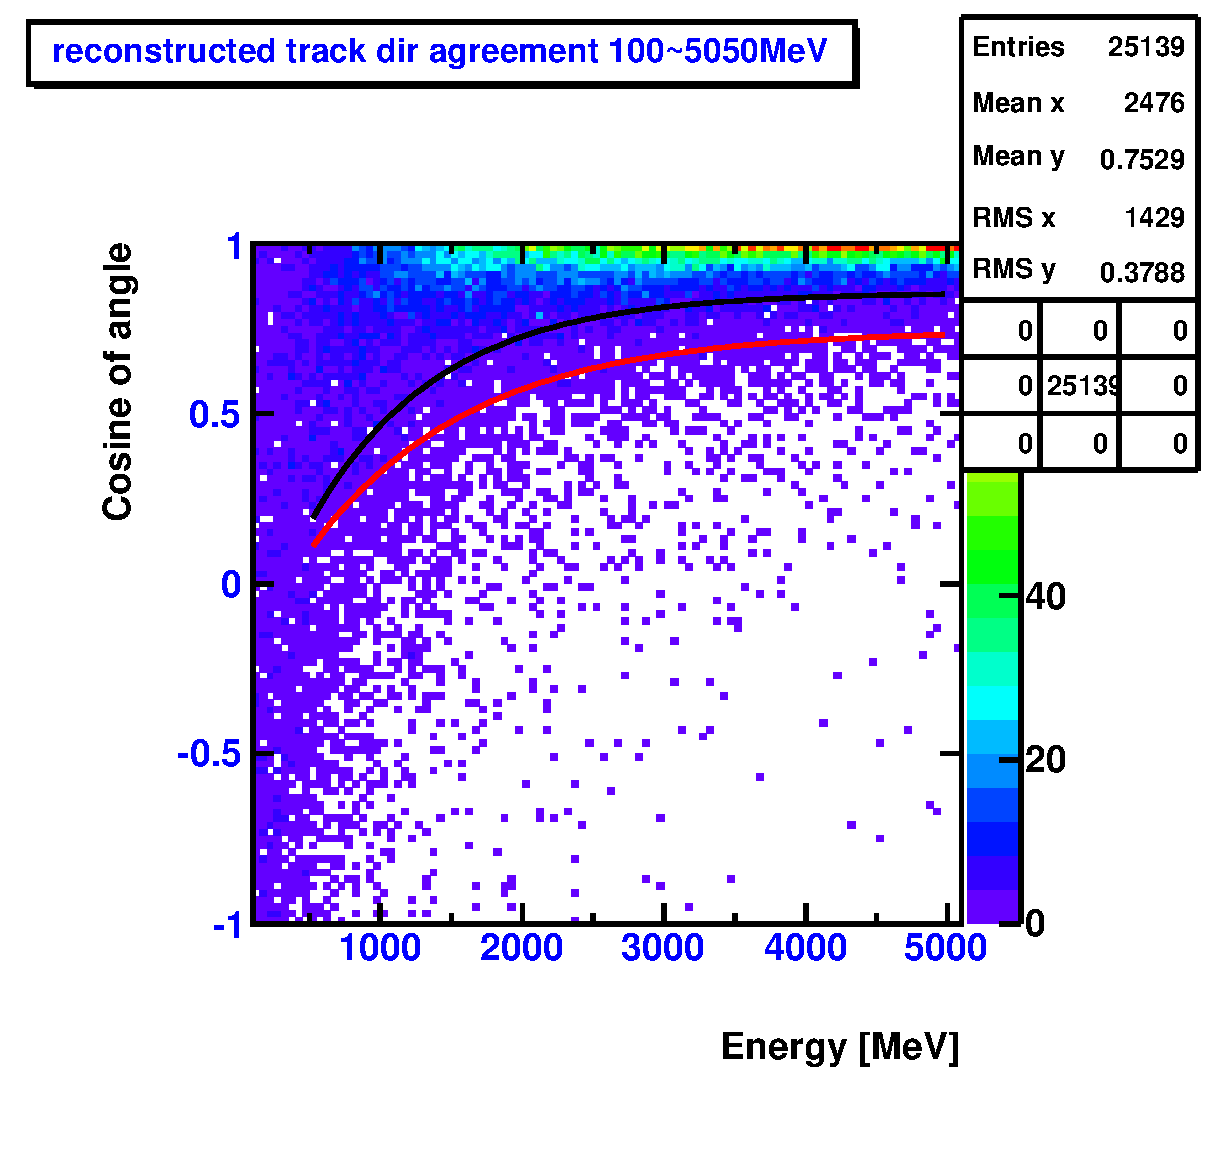
\includegraphics[width=1.0\textwidth]{material/nue_C12/analyzed_mtq_flatSpectrum_nue_C12_outerBufferFillAll_reconDirAgreementWithMtqTruthVectorVSEnergy_onlyCC_maxR600cm.eps}
	\end{columns}
\end{frame}

\begin{frame}
	\begin{itemize}
		\item Direction reconstruction is improved by fiductial volume cut on
			reconstructed vertex.
		\item What does the vertex mean for an finite size track shape event?
	\end{itemize}
\end{frame}

\begin{frame}
	\frametitle{$e^{-}$ track length}
	\begin{center}
		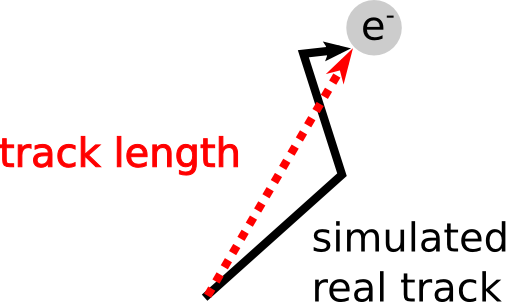
\includegraphics[height=0.2\textheight]{track_length_definition.png}
	\end{center}
	\begin{columns}[t]
		\column{0.5\textwidth}
		\ce{\nu_{e} + ^{1}H -> e^{-} + ?}
		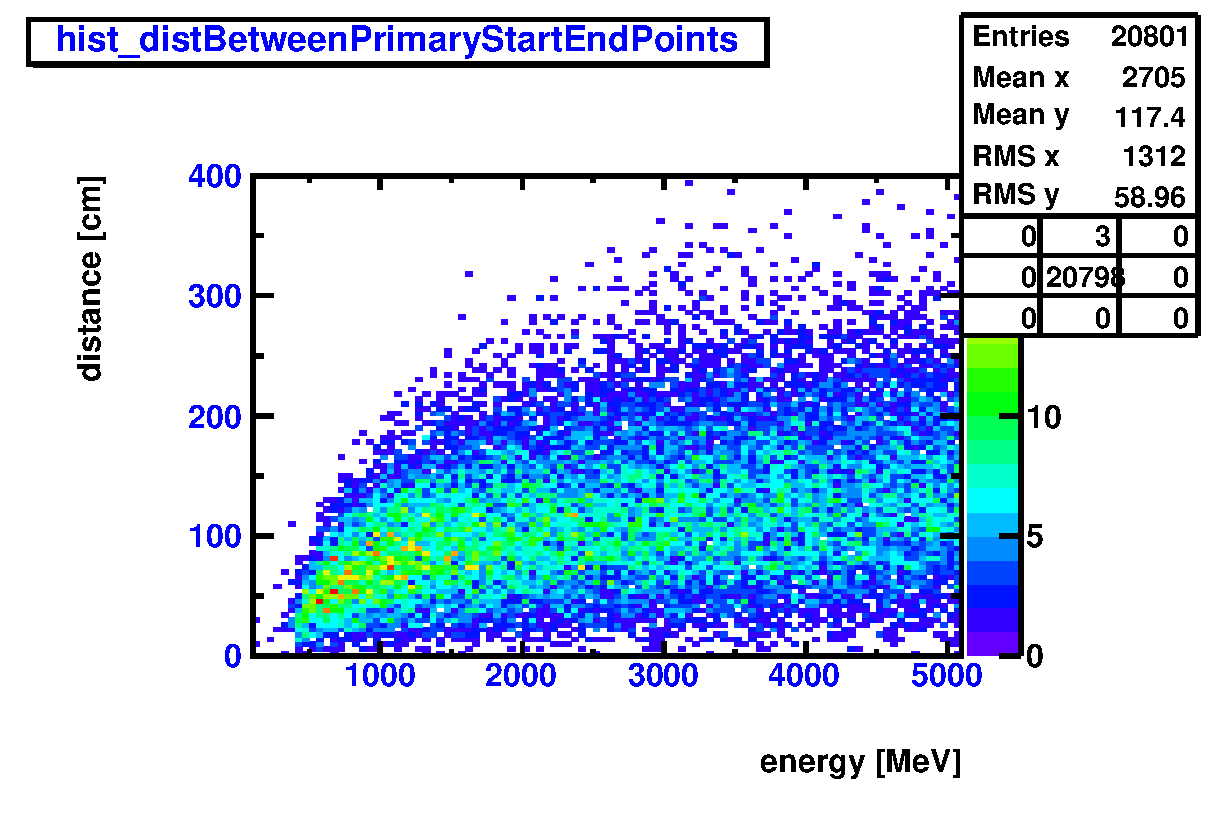
\includegraphics[width=1.0\textwidth]{nue_H1_distBetweenPrimaryStartEndPoints_onlyCC_maxR600cm.eps}
		\column{0.5\textwidth}
		\ce{\nu_{e} + ^{12}C -> e^{-} + ?}
		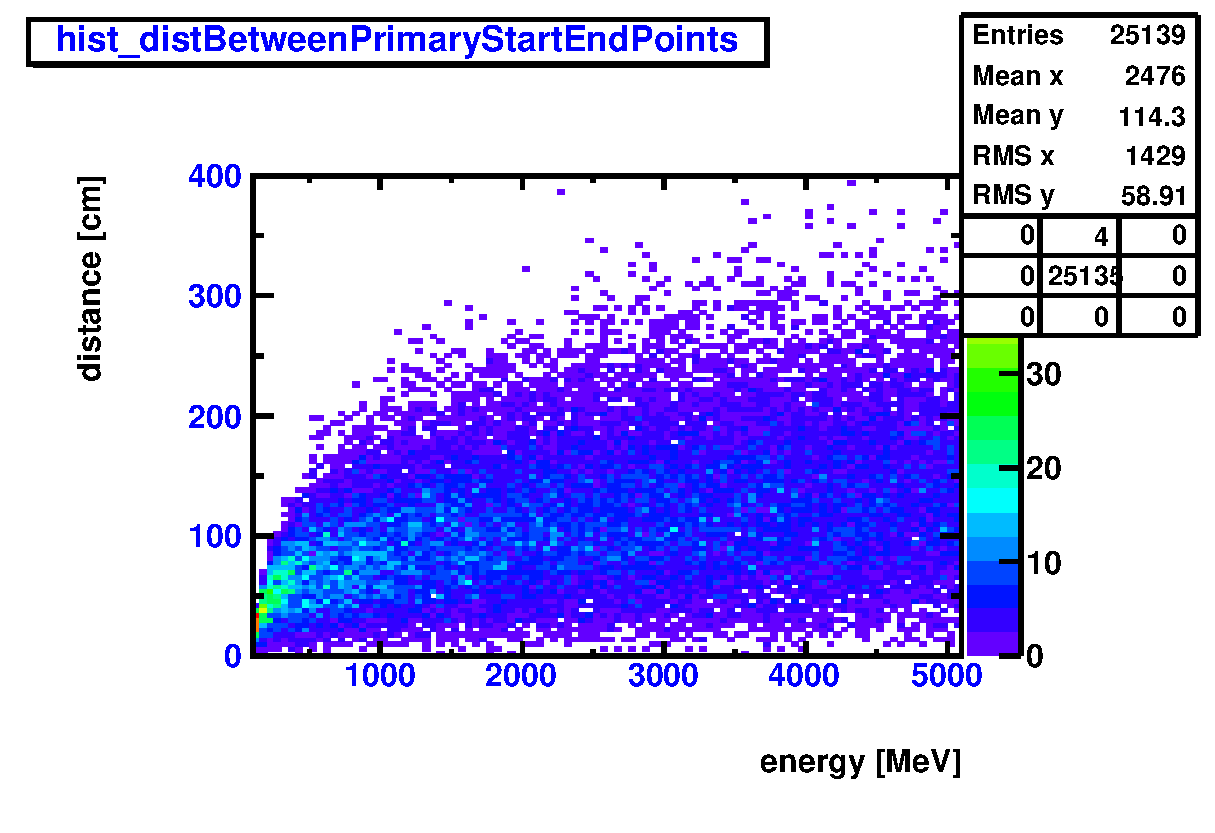
\includegraphics[width=1.0\textwidth]{nue_C12_distBetweenPrimaryStartEndPoints_onlyCC_maxR600cm.eps}
	\end{columns}
\end{frame}

\begin{frame}
	\frametitle{Perpendicular distance from reconstructed vertex to track}
	\framesubtitle{track using simulated track end points}
	\begin{center}
		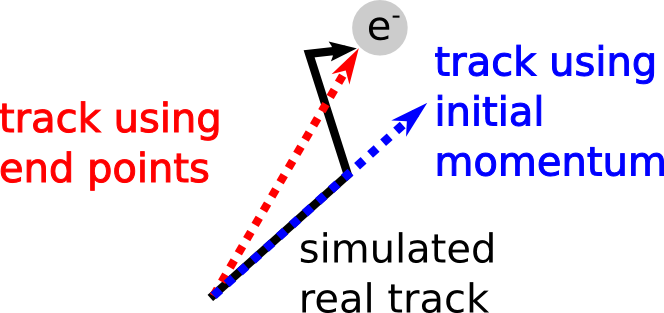
\includegraphics[height=0.2\textheight]{track_definition.png}
	\end{center}
	\begin{columns}[t]
		\column{0.5\textwidth}
		\ce{\nu_{e} + ^{1}H -> e^{-} + ?}
		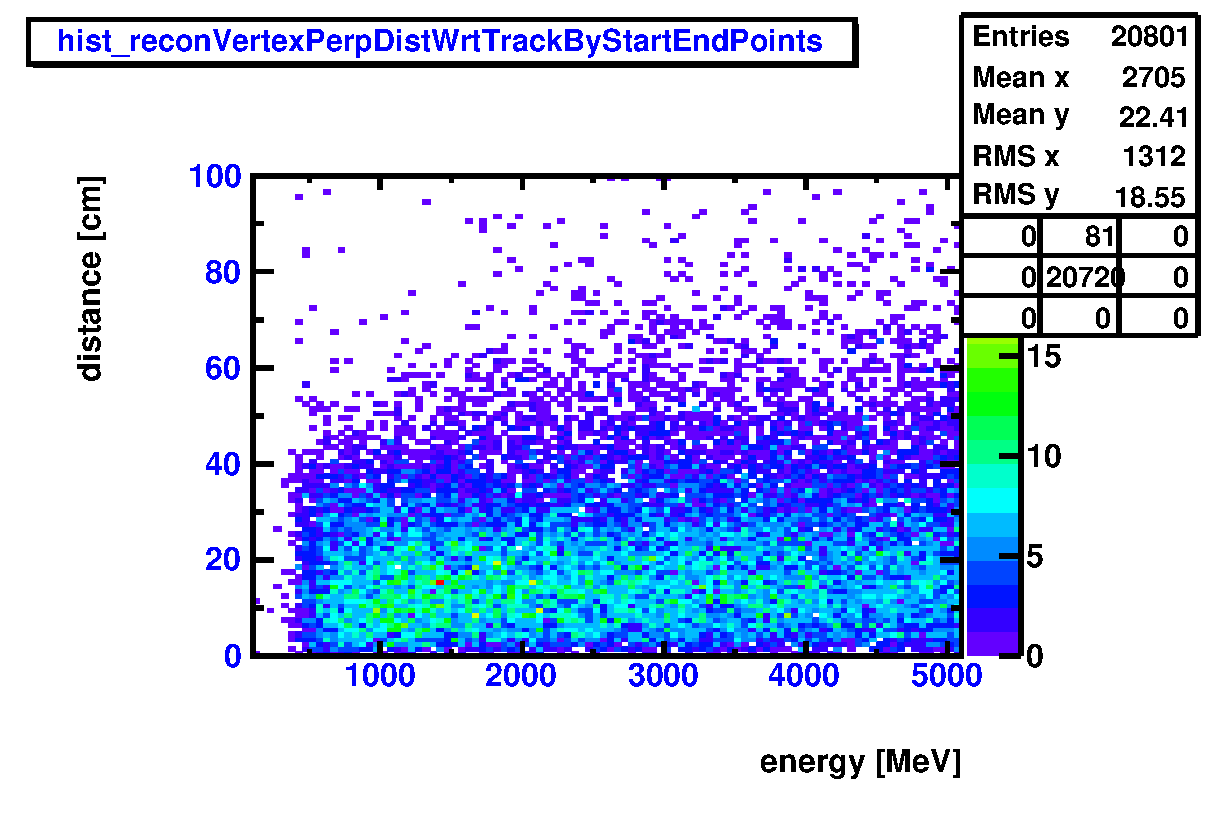
\includegraphics[width=1.0\textwidth]{nue_H1_reconVertexPerpDistWrtTrackByStartEndPoints_onlyCC_maxR600cm.eps}\\
		\column{0.5\textwidth}
		\ce{\nu_{e} + ^{12}C -> e^{-} + ?}
		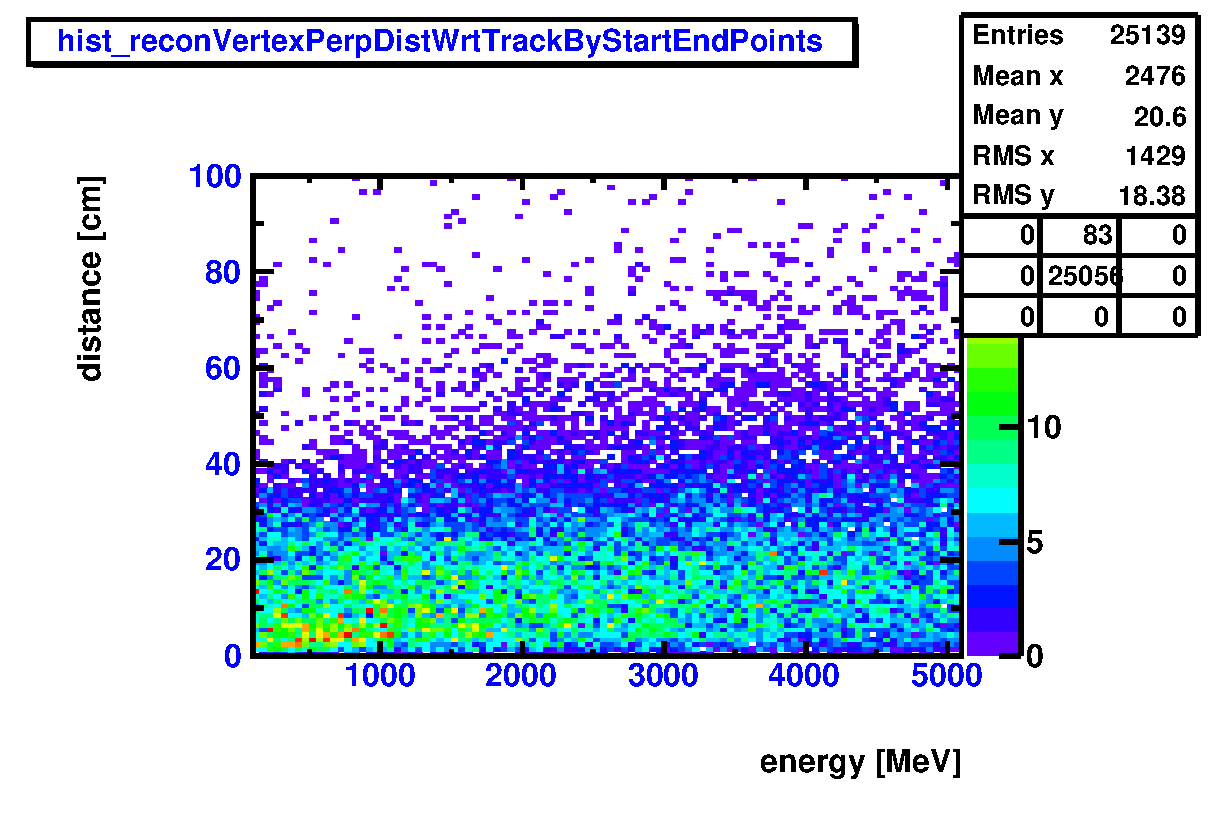
\includegraphics[width=1.0\textwidth]{nue_C12_reconVertexPerpDistWrtTrackByStartEndPoints_onlyCC_maxR600cm.eps}
	\end{columns}
\end{frame}

\begin{frame}
	\frametitle{Perpendicular distance from reconstructed vertex to track}
	\framesubtitle{track using simulated initial momentum}
	\begin{center}
		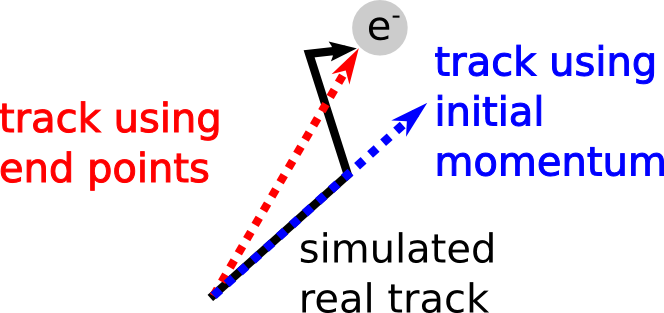
\includegraphics[height=0.2\textheight]{track_definition.png}
	\end{center}
	\begin{columns}[t]
		\column{0.5\textwidth}
		\ce{\nu_{e} + ^{1}H -> e^{-} + ?}
		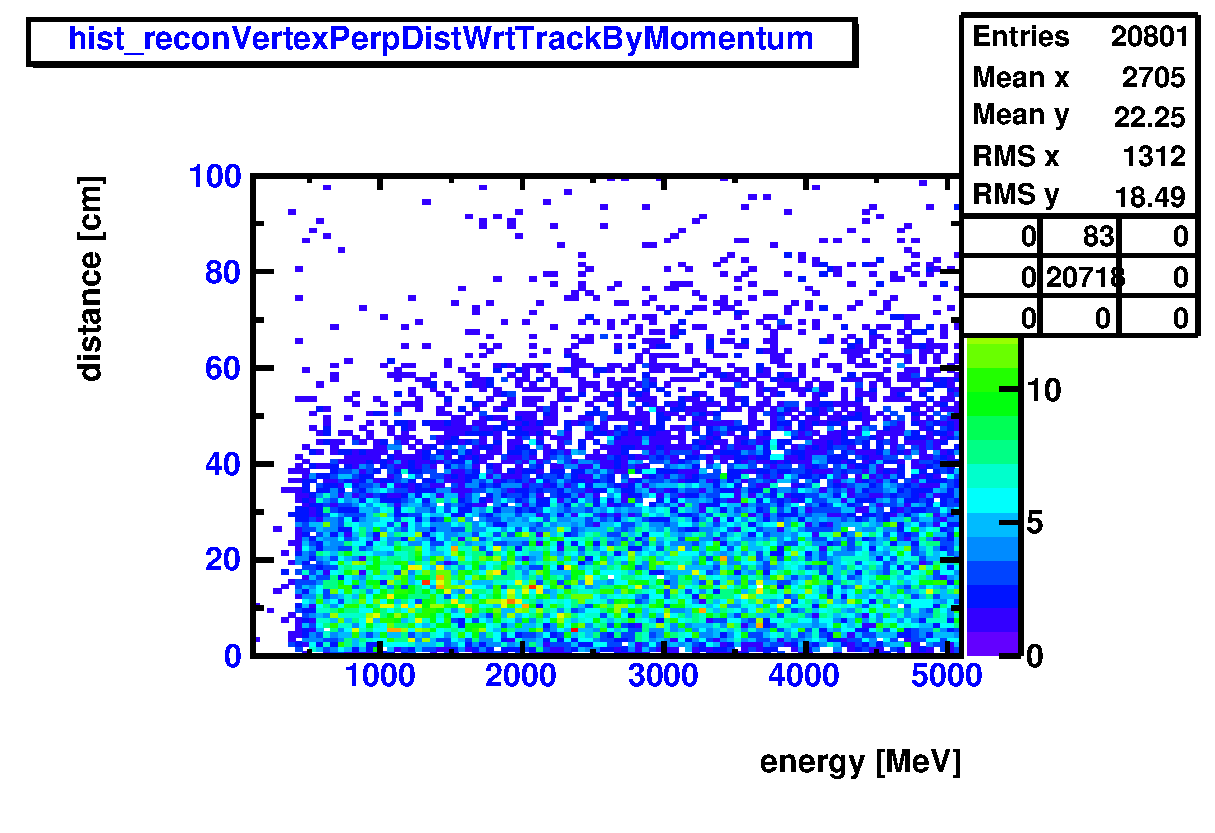
\includegraphics[width=1.0\textwidth]{nue_H1_reconVertexPerpDistWrtTrackByMomentum_onlyCC_maxR600cm.eps}
		\column{0.5\textwidth}
		\ce{\nu_{e} + ^{12}C -> e^{-} + ?}
		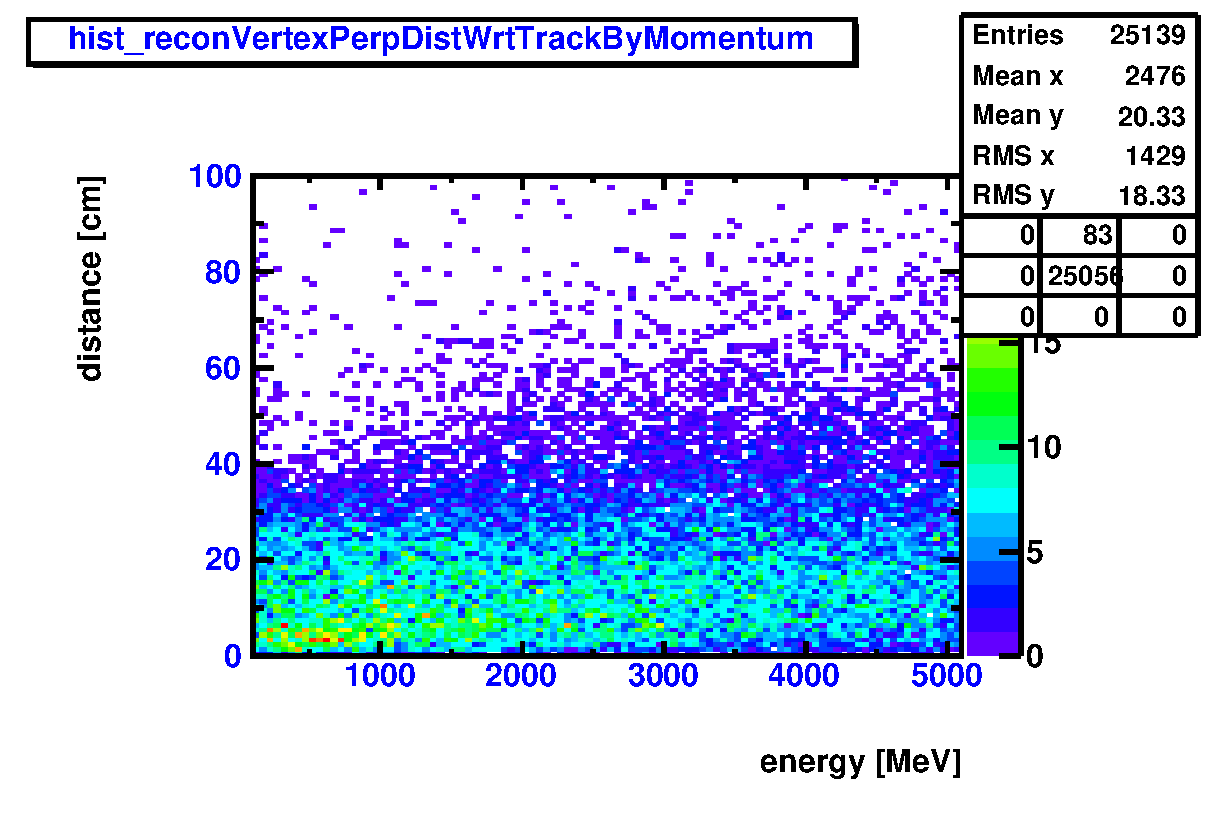
\includegraphics[width=1.0\textwidth]{nue_C12_reconVertexPerpDistWrtTrackByMomentum_onlyCC_maxR600cm.eps}
	\end{columns}
\end{frame}

\begin{frame}
	\frametitle{Distance of reconstructed vertex from track end points projected along tracks}
	\begin{center}
		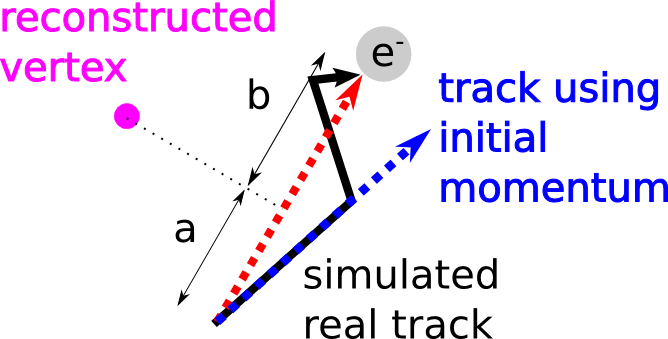
\includegraphics[height=0.4\textheight]{vertex_distance_definition.png}
	\end{center}
\end{frame}

\begin{frame}
	\frametitle{Distance of reconstructed vertex from track end points projected along tracks}
	\begin{tabular}{|C|V|V|}
		\hline
		&\ce{\nu_{e} + ^{1}H -> e^{-} + ?} &\ce{\nu_{e} + ^{12}C -> e^{-} + ?}\\
		\hline
		b &
		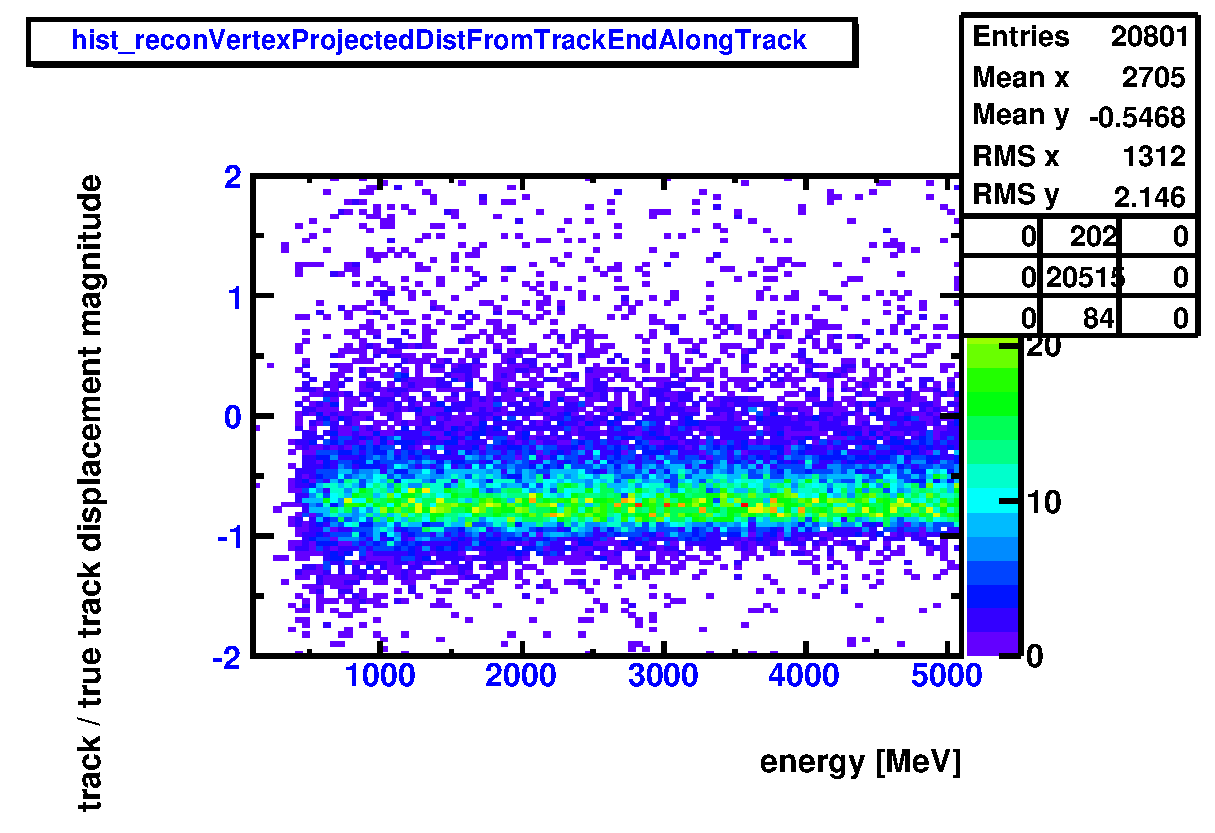
\includegraphics[width=0.45\textwidth]{nue_H1_reconVertexProjectedDistFromTrackEndAlongTrack_onlyCC_maxR600cm.eps} &
		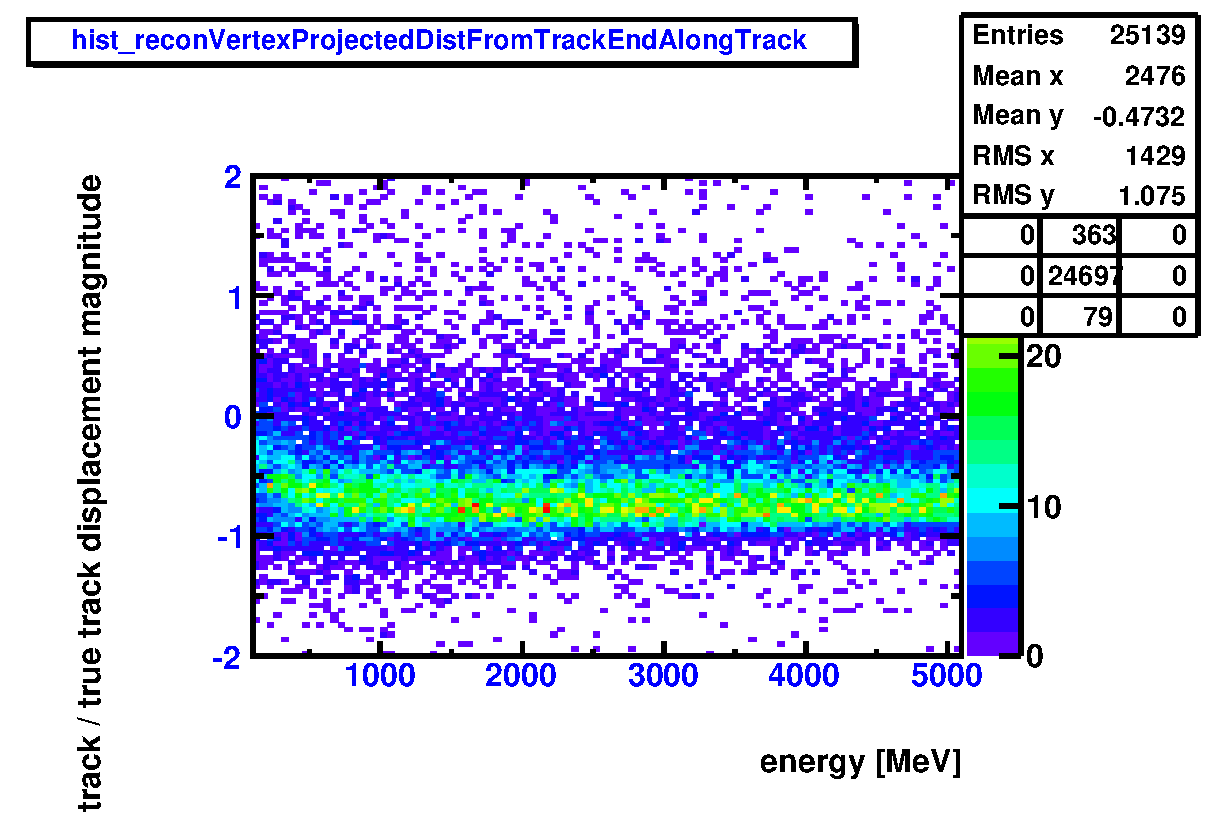
\includegraphics[width=0.45\textwidth]{nue_C12_reconVertexProjectedDistFromTrackEndAlongTrack_onlyCC_maxR600cm.eps} \\
		\hline
		a &
		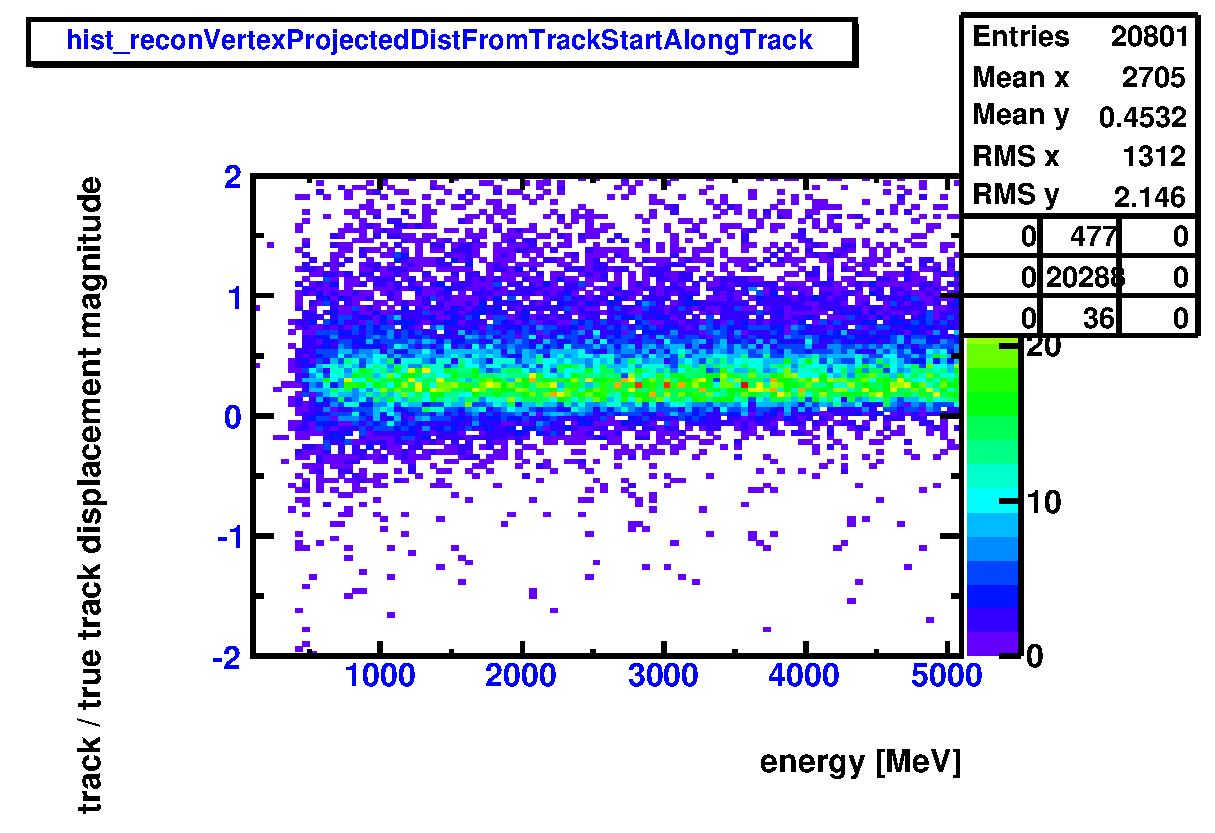
\includegraphics[width=0.45\textwidth]{nue_H1_reconVertexProjectedDistFromTrackStartAlongTrack_onlyCC_maxR600cm.eps} &
		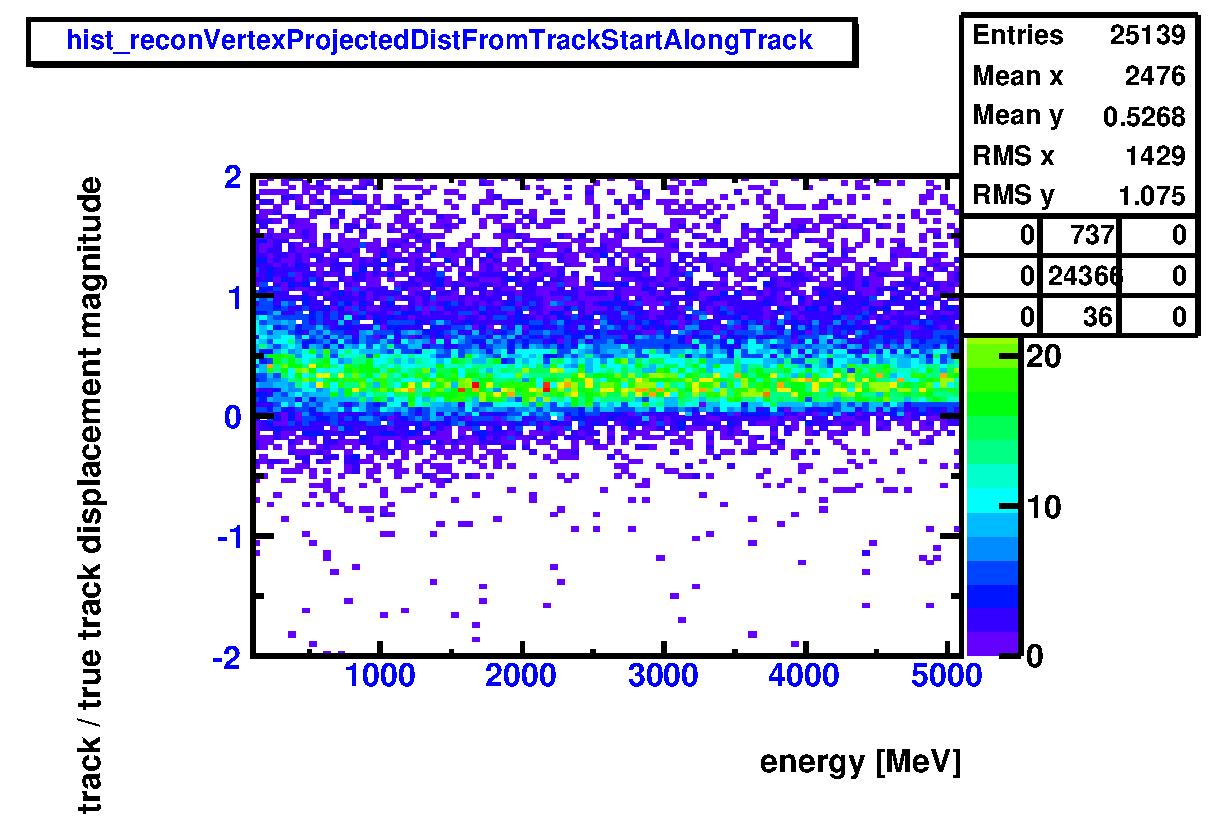
\includegraphics[width=0.45\textwidth]{nue_C12_reconVertexProjectedDistFromTrackStartAlongTrack_onlyCC_maxR600cm.eps} \\
		\hline
	\end{tabular}
\end{frame}

\begin{frame}
	\frametitle{Conclusion for reconstruction vertex}
	For $\nu$ energies \SIrange{100}{5000}{MeV}:
	\begin{itemize}
		\item Vertex is within ~40cm from track
		\item Vertex is on average at ~middle of track
		\item peak of vertex distribution is biased toward track beginning.
	\end{itemize}
\end{frame}

\begin{frame}
	\frametitle{Lepton energy vs true $\nu$ energy}
	\begin{columns}[t]
		\column{0.5\textwidth}
		\ce{\nu_{e} + ^{1}H -> e^{-} + ?}
		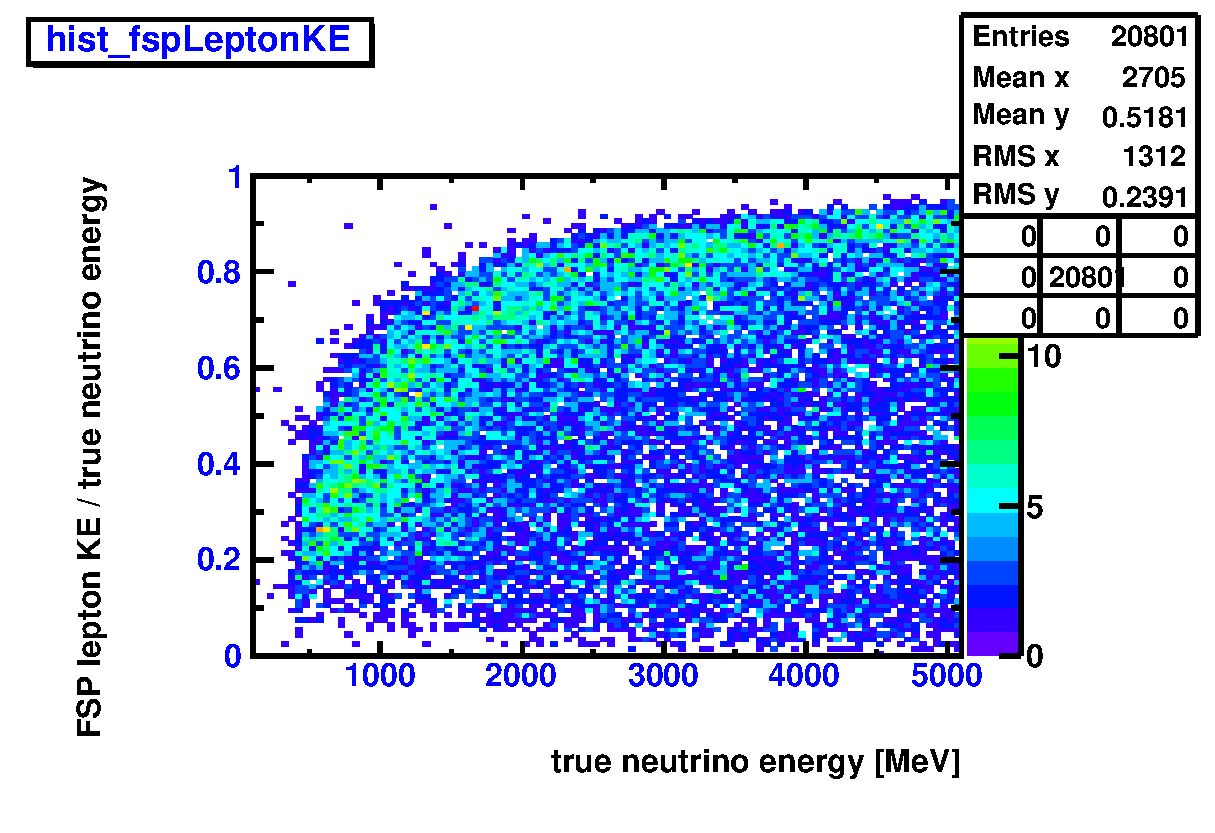
\includegraphics[width=1.0\textwidth]{nue_H1_fspLeptonVSTrueNuEnergy_onlyCC_maxR600cm.eps}
		\column{0.5\textwidth}
		\ce{\nu_{e} + ^{12}C -> e^{-} + ?}
		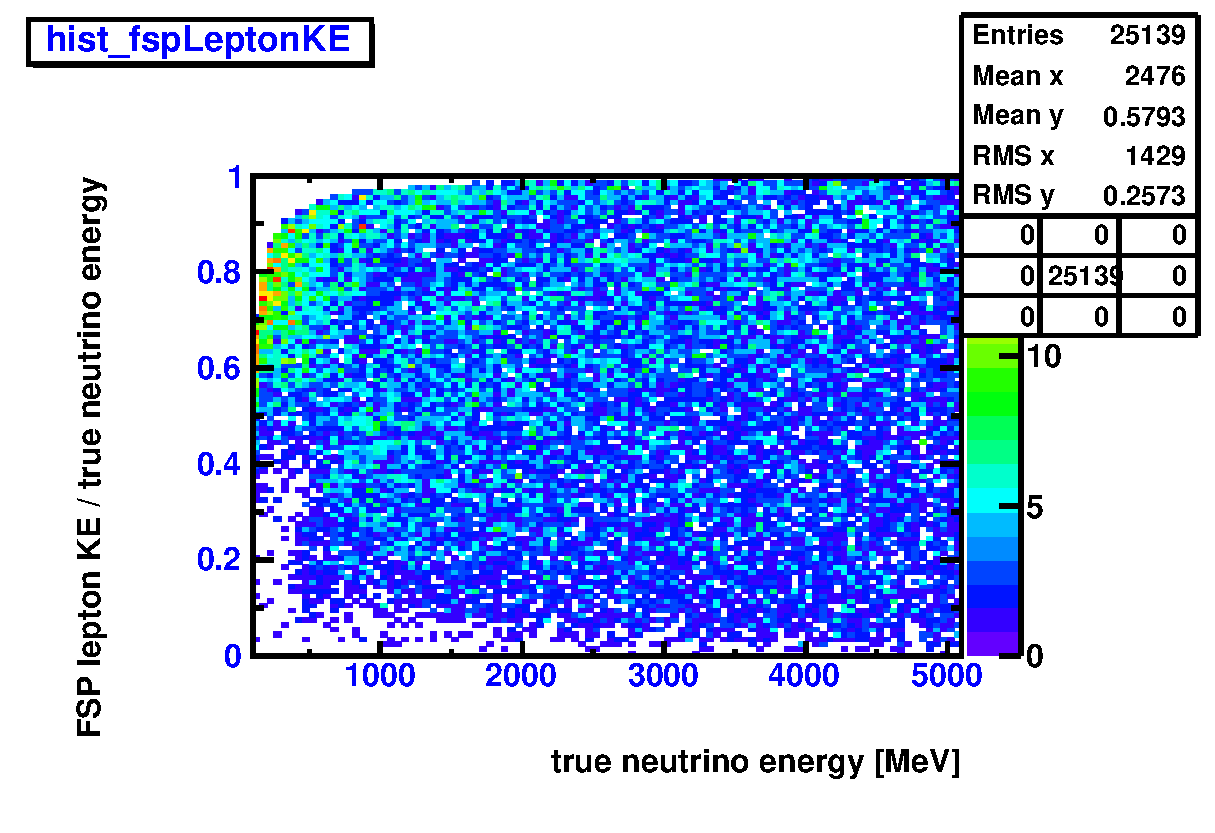
\includegraphics[width=1.0\textwidth]{nue_C12_fspLeptonVSTrueNuEnergy_onlyCC_maxR600cm.eps}
	\end{columns}
\end{frame}

\begin{frame}
	\frametitle{Total charge vs true $\nu$ energy}
	\begin{columns}[t]
		\column{0.5\textwidth}
		\ce{\nu_{e} + ^{1}H -> e^{-} + ?}
		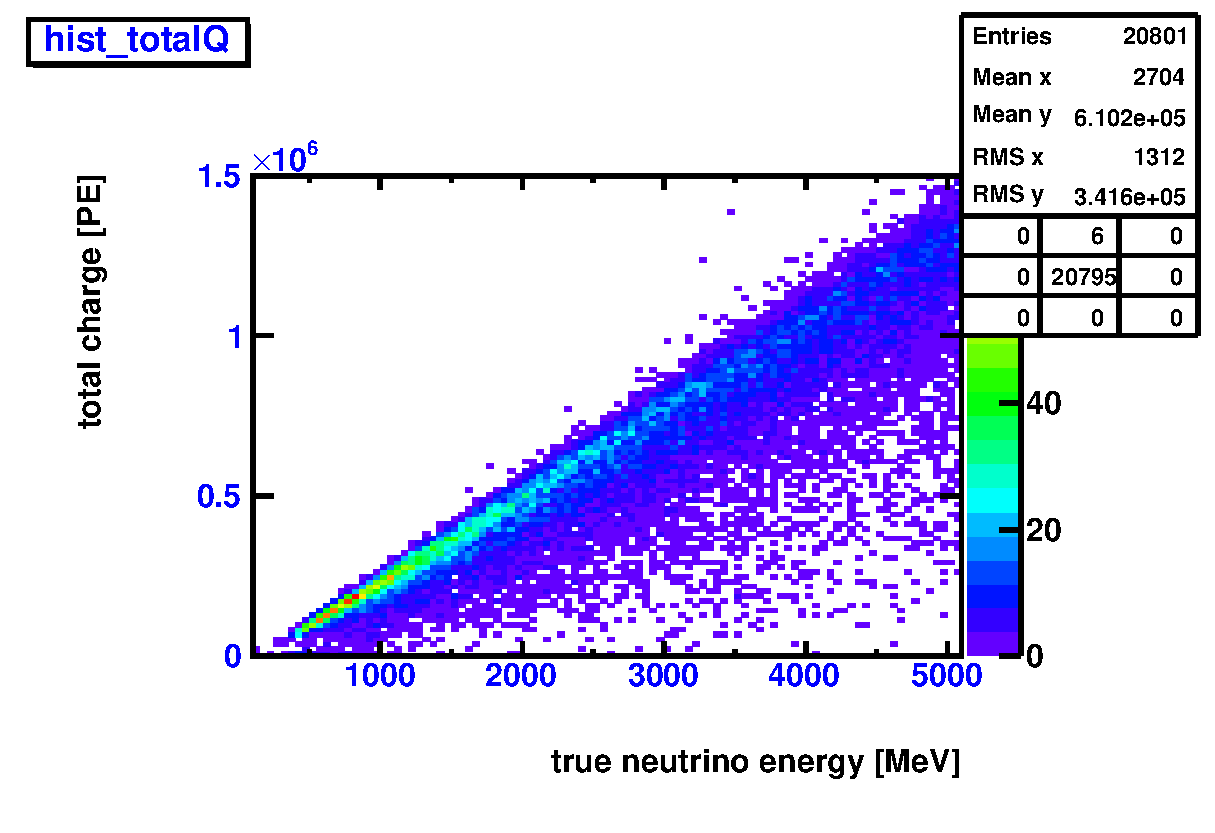
\includegraphics[width=1.0\textwidth]{nue_H1_totalChargeVSTrueNuEnergy_onlyCC_maxR600cm.eps}
		\column{0.5\textwidth}
		\ce{\nu_{e} + ^{12}C -> e^{-} + ?}
		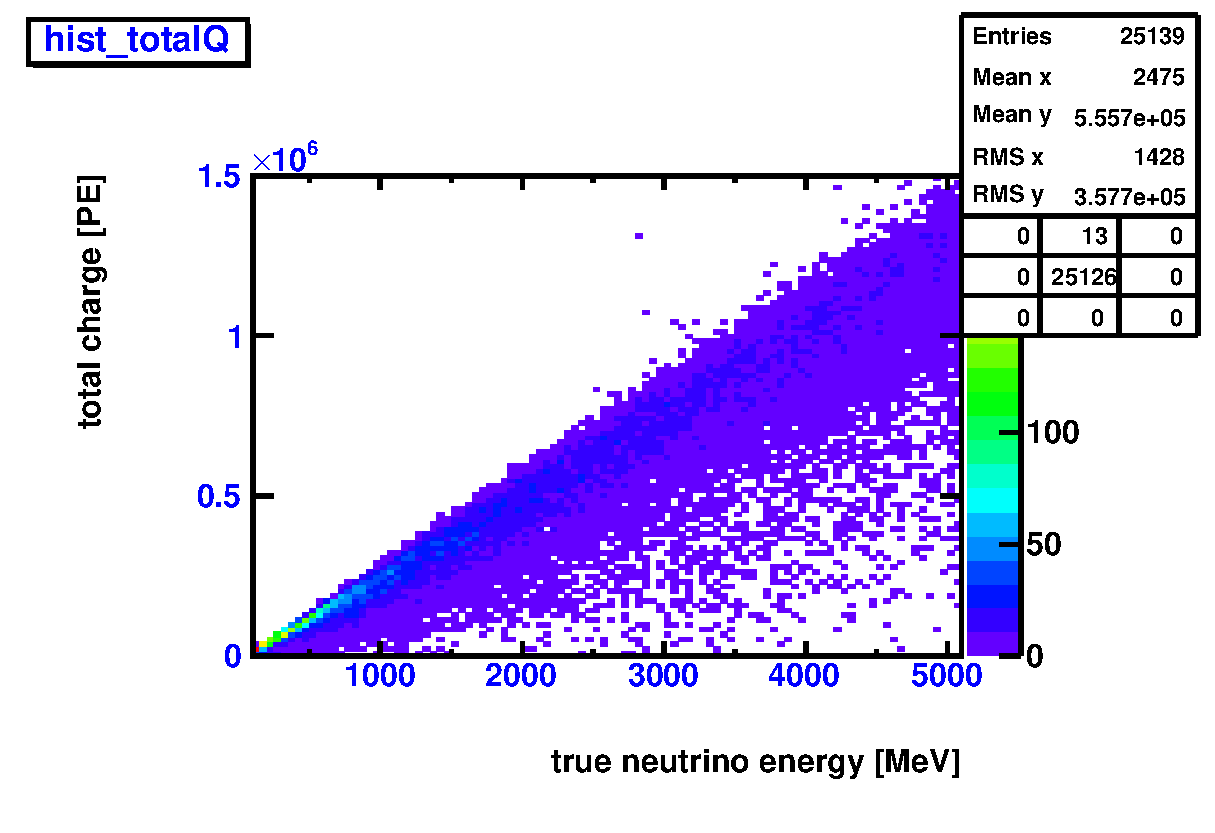
\includegraphics[width=1.0\textwidth]{nue_C12_totalChargeVSTrueNuEnergy_onlyCC_maxR600cm.eps}
	\end{columns}
\end{frame}

\begin{frame}
	\frametitle{Reconstructed vs true $\nu$ energy}
	\begin{columns}[t]
		\column{0.5\textwidth}
		\ce{\nu_{e} + ^{1}H -> e^{-} + ?}
		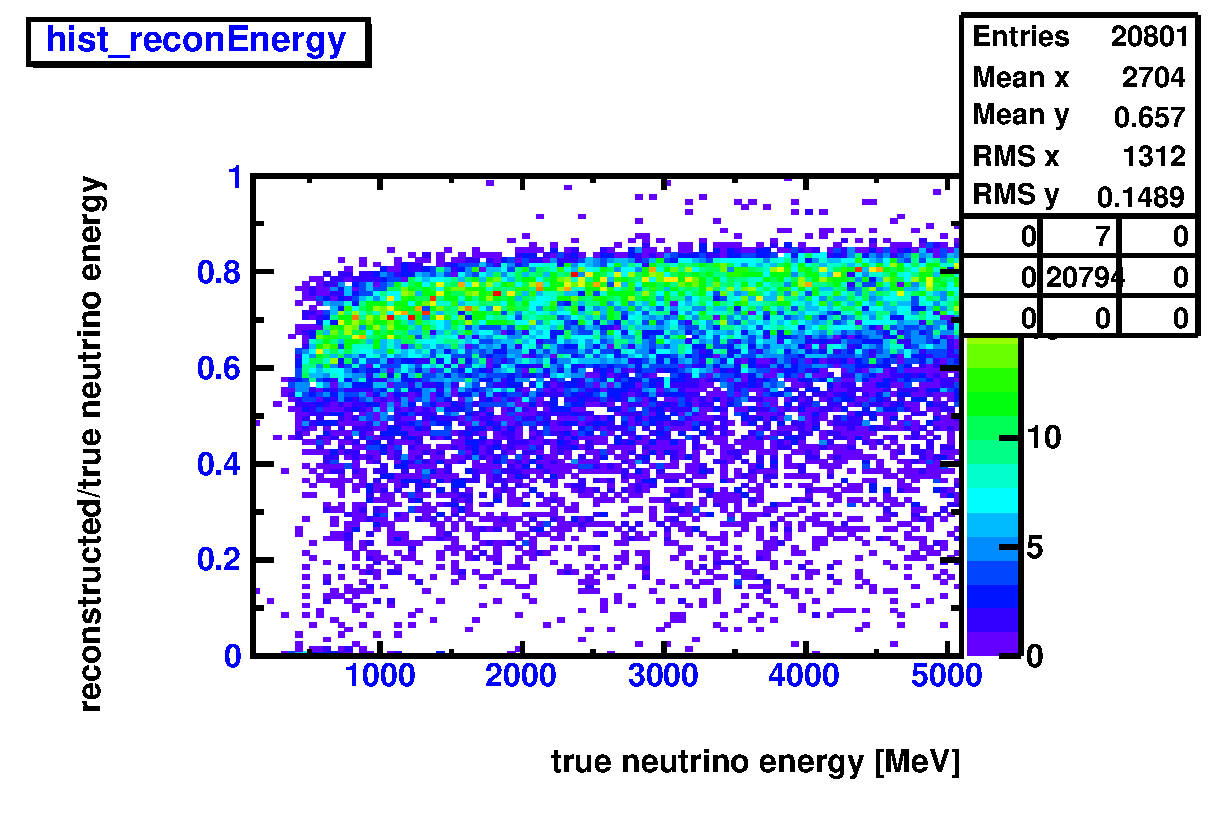
\includegraphics[width=1.0\textwidth]{nue_H1_reconVSTrueNuEnergy_onlyCC_maxR600cm.eps}
		\column{0.5\textwidth}
		\ce{\nu_{e} + ^{12}C -> e^{-} + ?}
		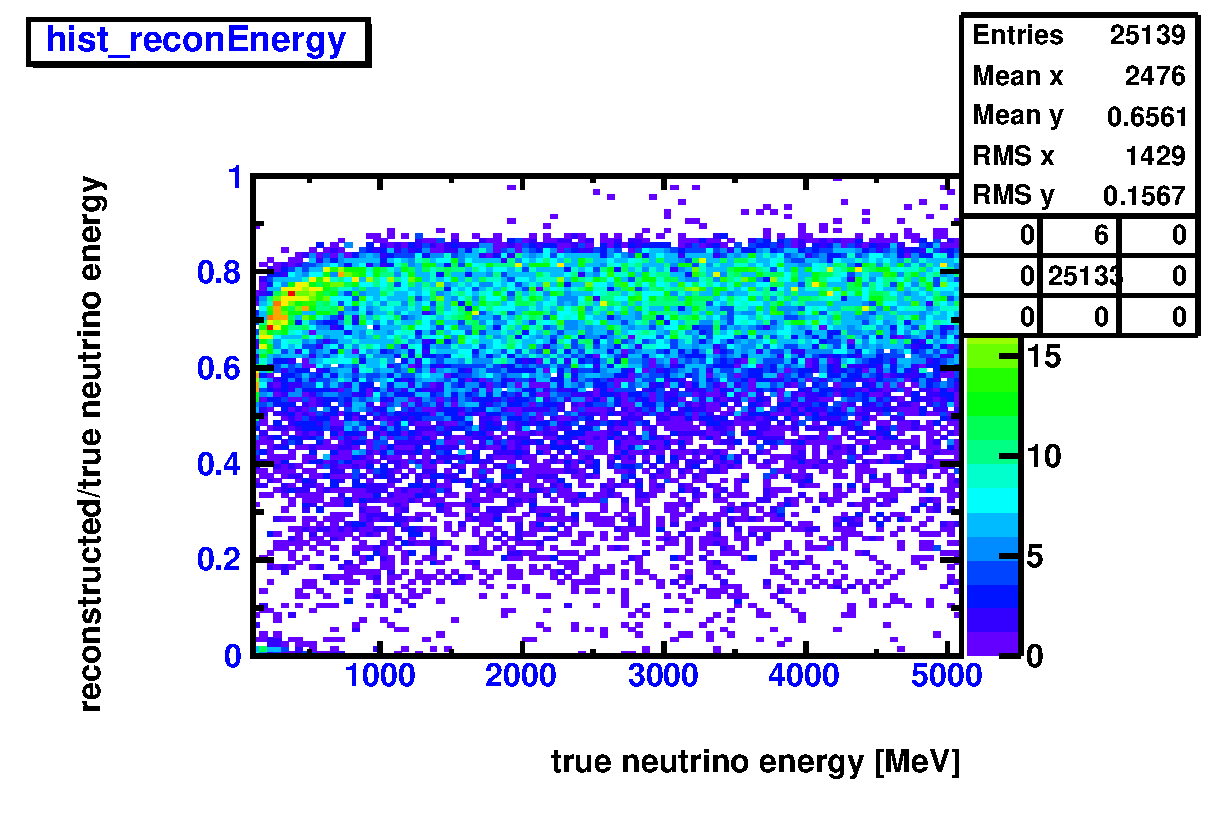
\includegraphics[width=1.0\textwidth]{nue_C12_reconVSTrueNuEnergy_onlyCC_maxR600cm.eps}
	\end{columns}
	Consistently $80\%$ of energy is reconstructed for extremely large energy range.
\end{frame}

\begin{frame}
	\frametitle{Pion energy loss in nucleus?}
	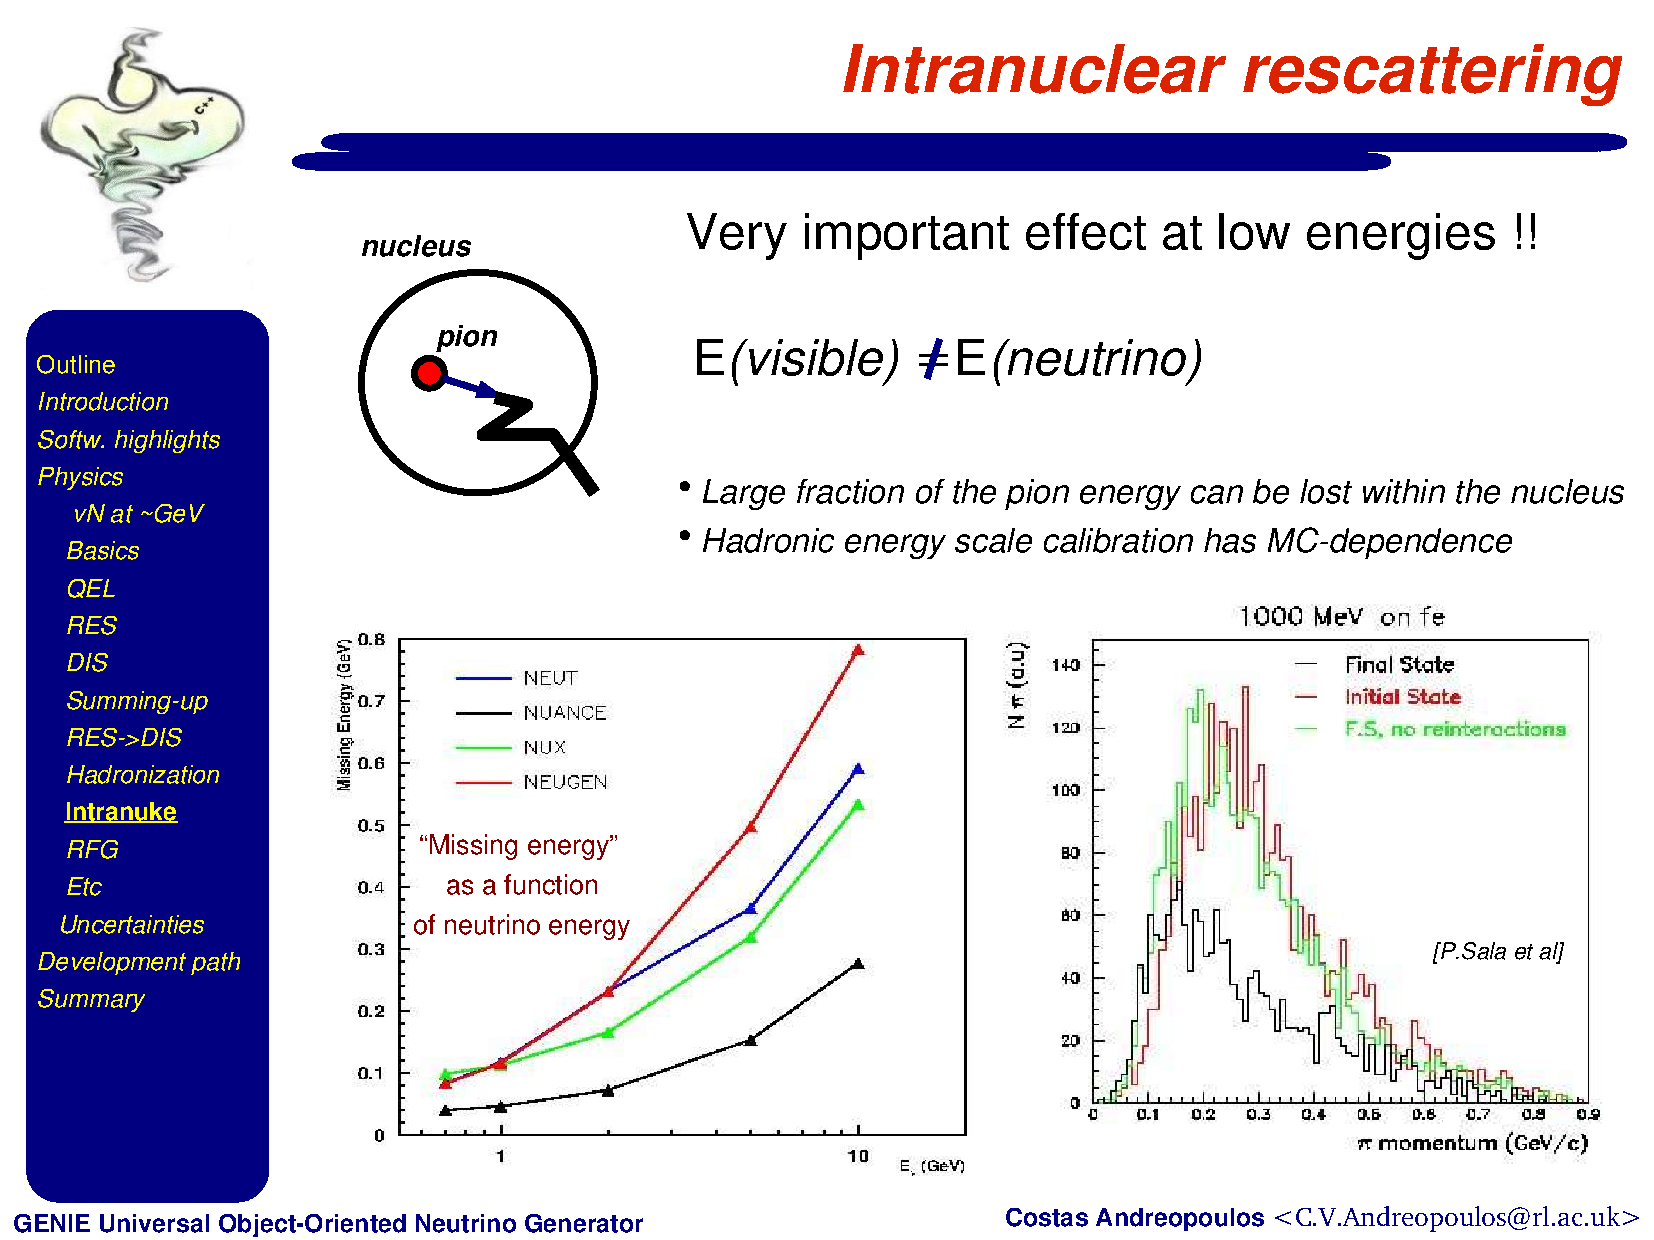
\includegraphics[width=\textwidth]{genie_pi_energy_loss.pdf}
\end{frame}

\end{document}
